\documentclass[letterpaper, reqno,11pt]{article}
\usepackage[margin=1.0in]{geometry}
\usepackage{color,latexsym,amsmath,amssymb,graphicx,float,listings,tikz}
\usepackage{hyperref}

\hypersetup{
colorlinks=true,
linkcolor=magenta,
filecolor=magenta,
urlcolor=cyan,
}

\lstset{
basicstyle=\ttfamily,
columns=fullflexible,
frame=single,
breaklines=true,
postbreak=\mbox{\textcolor{red}{$\hookrightarrow$}\space},
}

\graphicspath{ {images/} }

\begin{document}
\pagenumbering{arabic}
\title{PHYS408 Homework 2}
\date{13/02/24}
\author{Xander Naumenko}
\maketitle

{\medskip\noindent\bf Question 1a.} In class, we derived the following result in the Fraunhofer limit:
\[
    E(x',y')\approx \frac{e^{ikz}}{i\lambda z}e^{ik \frac{x'^2+y'^2}{2z}}\tilde E(k_x,k_y)
.\]
Thus all we have to do is compute the Fourier transform of the two slits. We can describe the slits as two shifted rectangles (assuming the input field $E$ is uniform and has magnitude 1):
\[
E(x,y) = \text{rect}\left(\frac{x}{d_x}\right)\left( \text{rect}\left( \frac{y-\Delta /2}{d_y} \right) +\text{rect}\left( \frac{y+\Delta /2}{d_y} \right)  \right) 
.\]
Also recall the following transform:
\[
    \mathcal F(\text{rect}(ax))=\frac{1}{|a|}\text{sinc}\left( \frac{k_x}{a} \right) 
.\]
Using this we get the following:
\[
    \tilde E(k_x, k_y) = d_xd_y \text{sinc}\left(\frac{d_xk_x}{2\pi}\right)\text{sinc}\left(\frac{d_yk_y}{2\pi}\right)\left( e^{i\Delta k_y /2}+e^{-i\Delta k_y /2} \right) 
.\]
Intensity is proportional to electric field squared, and since the question just asks for the distribution the constant factors can be discarded:
\[
I(x',y') \propto |E(x',y')|^2=\frac{1}{(\lambda z)^2} \text{sinc}^2\left(\frac{d_xk_x}{2\pi}\right)\text{sinc}^2\left(\frac{d_yk_y}{2\pi}\right)\sin^2\left( \frac{\Delta k_y}{2} \right) 
\]
where as usual $k_x= \frac{kx'}{z}$ and $k_y=\frac{ky'}{z}$.

{\medskip\noindent\bf Question 1b.} See figure \ref{fig:q1b}. The code used to produced the graphs is here:
\begin{lstlisting}
import numpy as np
import matplotlib.pyplot as plt

dx = 0.01
dy = 0.001
delta = 0.005
lam = 500e-9
z = 50

k = 2*np.pi/lam

x = np.linspace(-0.05, 0.05, 1000)
y = np.linspace(-0.05, 0.05, 1000)

kx = k*x/z
ky = k*y/z

Ix = (lam/z*np.sinc(dx*kx/(4*np.pi)))**2
Iy = (lam/z*np.sinc(dy*ky/(4*np.pi))*np.sin(delta*ky/2))**2

plt.plot(x, Ix)
plt.title("Intensity of Double Slit for y=0 Axis")
plt.xlabel("x' (m)")
plt.ylabel("I (W/m$^2$)")
plt.show()

plt.plot(y, Iy)
plt.title("Intensity of Double Slit for x=0 Axis")
plt.xlabel("y' (m)")
plt.ylabel("I (W/m$^2$)")

plt.show()
\end{lstlisting}

\begin{figure}[htpb]
    \centering
    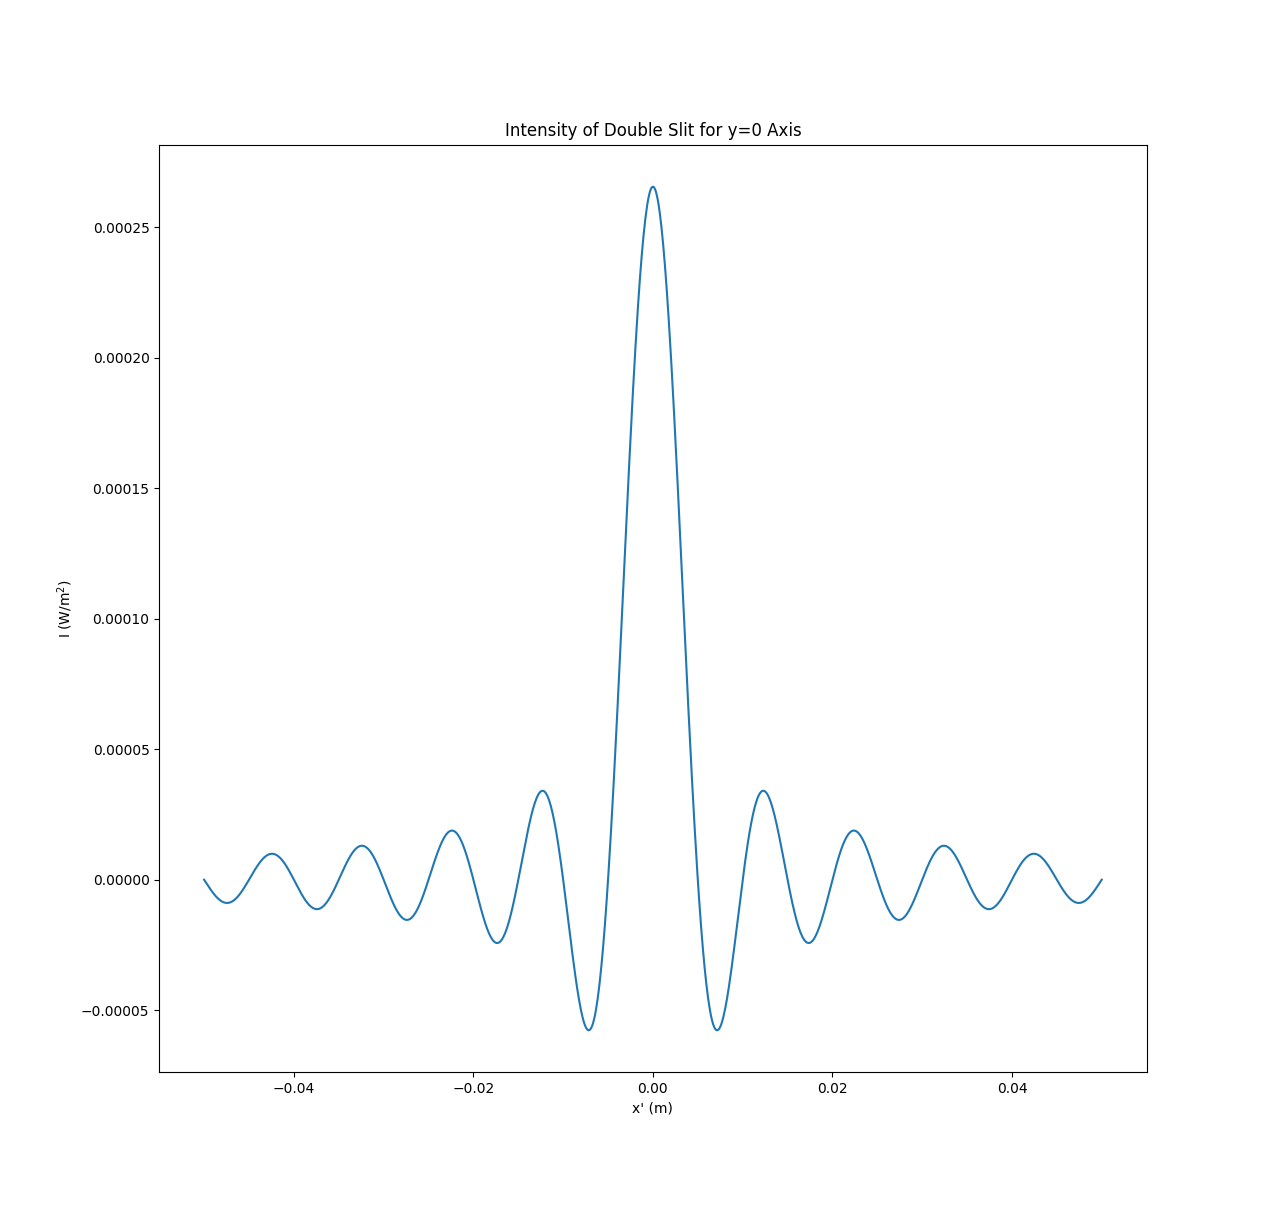
\includegraphics[width=0.6\textwidth]{q1x}
    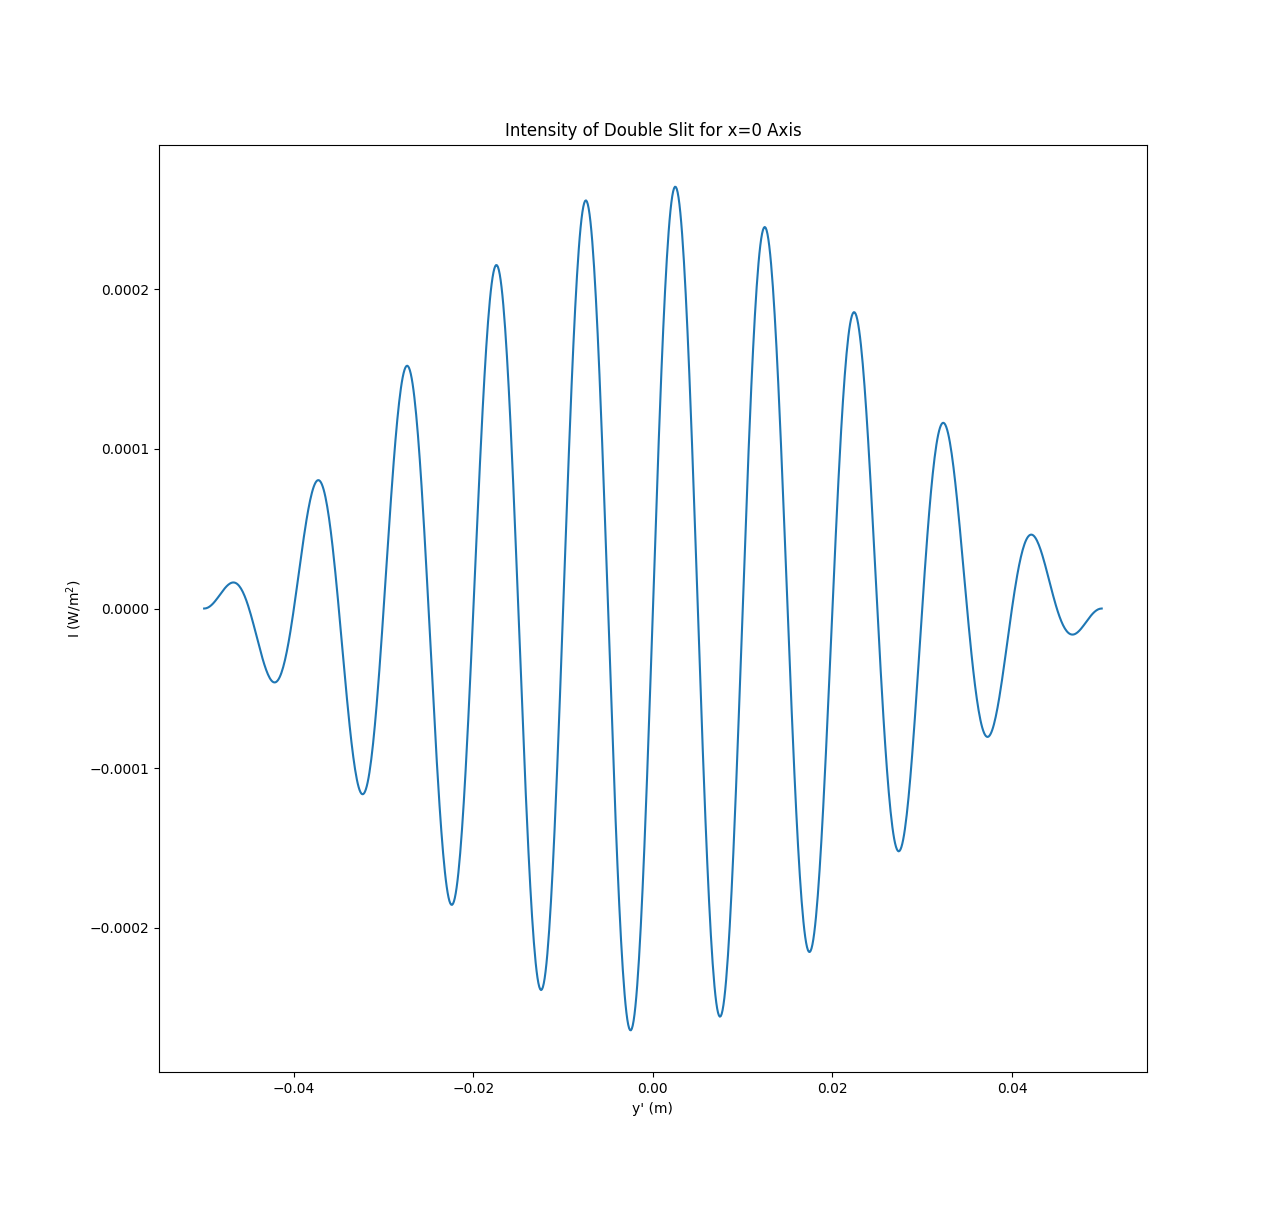
\includegraphics[width=0.6\textwidth]{q1y}
    \caption{Graphs for question 1b.}
    \label{fig:q1b}
\end{figure}

{\medskip\noindent\bf Question 1c.} The Fraunhofer limit applies only if $\frac{x^2}{\lambda}, \frac{y^2}{\lambda} \ll \frac{z}{\pi}$. In our case, these are $\frac{(d_x/2)^2}{\lambda}=50$ and $\frac{(d_y /2)^2}{\lambda}=\frac{1}{2}$. In comparison to $\frac{z}{\pi}\approx 15.9$, we see that the $x$-axis is no in the Fraunhofer approximation, so our results above are not totally valid.

{\medskip\noindent\bf Question 1d.} 


% {\medskip\noindent\bf Question 2a.} Width the addition of the finite length, the thickness function is 
% \[
%     d(x)=\left( \overline{d}+\frac{d_0}{2} \sin\left( 2\pi x /\Lambda \right)  \right)\text{rect}(x /d_x)
% .\]
% The Fourier transform of the left hand side is 

{\medskip\noindent\bf Question 2a.} The phase function is going to be proportional to the thickness, so assuming no transmission occurs outside of $d_x$, we have
\[
t(x) = \text{rect}\left(\frac{x}{d_x}\right)e^{ikn\left(\overline{d}+\frac{d_0}{2}\sin(2\pi x /\Lambda)\right)}e^{-ik \frac{d_0}{2}\sin\left( 2\pi x /\Lambda \right) }=\text{rect}\left(\frac{x}{d_x}\right)e^{ikn\overline{d}+ik(n-1)\frac{d_0}{2}\sin(2\pi x /\Lambda)}
.\]

{\medskip\noindent\bf Question 2b.} The incoming plane wave can be represented as $E=E_0 e^{ik\theta_i x}$. Thus the transmitted waves are:
\[
E_t(x)=E(x)\cdot t(x)E_0 e^{ik\theta_i x} e^{ikn\overline{d}+ik(n-1)\frac{d_0}{2}\sin(2\pi x /\Lambda)}
\]
\[
=E_0\sum_{q=-\infty}^{\infty}J_q\left(k(n-1) \frac{d_0}{2}\right)e^{i 2\pi qx /\Lambda+ik\theta_ix+ikn\overline{d}}
\]
\[
=E_0'\sum_{q=-\infty}^{\infty}J_q\left(k(n-1) \frac{d_0}{2}\right)e^{i 2\pi qx /\Lambda+ik\theta_ix} 
\]
\[
=E_0'\sum_{q=-\infty}^{\infty}J_q\left(k(n-1) \frac{d_0}{2}\right)e^{ikx(\lambda qx /\Lambda+\theta_i)} 
.\]
This is exactly an infinite combination of plane waves with angles $\theta_q=\theta_i+\frac{q\lambda}{\Lambda}$, as required.

{\medskip\noindent\bf Question 3.} For the image plane to be a reproduction of the original object, the transfer function of the whole system between the object plane and the image plane must be be a constant (there can potentially be a constant factor scaling, but there can't be any $x,y$ dependent phase terms). There are three optical components in play: the free space before the lens, the lens, and the free space after the lens. Ignoring the constant factors since they're not relevant, the total transfer function is then:
\[
    H(x',y')\propto e^{-i \frac{k}{2}(x'^2+y'^2) \frac{1}{d_o}}e^{-i \frac{k}{2}(x'^2+y'^2) \frac{1}{d_i}}e^{i \frac{k}{2}(x'^2+y'^2) \frac{1}{f}}=e^{-i \frac{k}{2}(x'^2+y'^2)\left( \frac{1}{d_0}+\frac{1}{d_i}-\frac{1}{f} \right) }
.\]
The only way that there is no $x',y'$ dependence is if the rightmost bracketed term is 0, which gives:
\[
\frac{1}{d_o}+\frac{1}{d_i}=\frac{1}{f}
.\]

{\medskip\noindent\bf Question 4.} From lecture, we know that the $E(x',y')\propto \mathcal F(\overline{E}(x,y))$, so if we want $E(x',y')$ to be proportional to $\tilde t(x,y)$, we need $\overline{E}$ to have a small phase factor. The expression for $\overline{E}$ is
\[
\overline{E}=E_0 t_0(x,y) e^{-i \frac{k}{2}(x^2+y^2)\left( \frac{1}{f}-\frac{1}{f-\Delta} \right) }
.\]
Since $\Delta \ll f$, we can say $\frac{1}{f}-\frac{1}{f-\Delta}= -\frac{\Delta}{f(f-\Delta)}\approx \frac{\Delta}{f^2}$. The Fourier transform of $\overline{E}$ only turns into $\tilde t(x,y)$ if the phase factor is very small while $x^2+y^2<D^2$, which occurs when $\frac{k}{2}(x^2+y^2) \frac{\Delta}{f^2}\ll 1\implies \Delta \ll \frac{2f^2}{kD^2}$.


\end{document}
